\section{Appendix C: Supplementary Signal-Layer Results}

This appendix presents additional material for the investor-oriented warning layer.

\subsection{Signal figures by asset}

\begin{figure}[H]
    \centering
    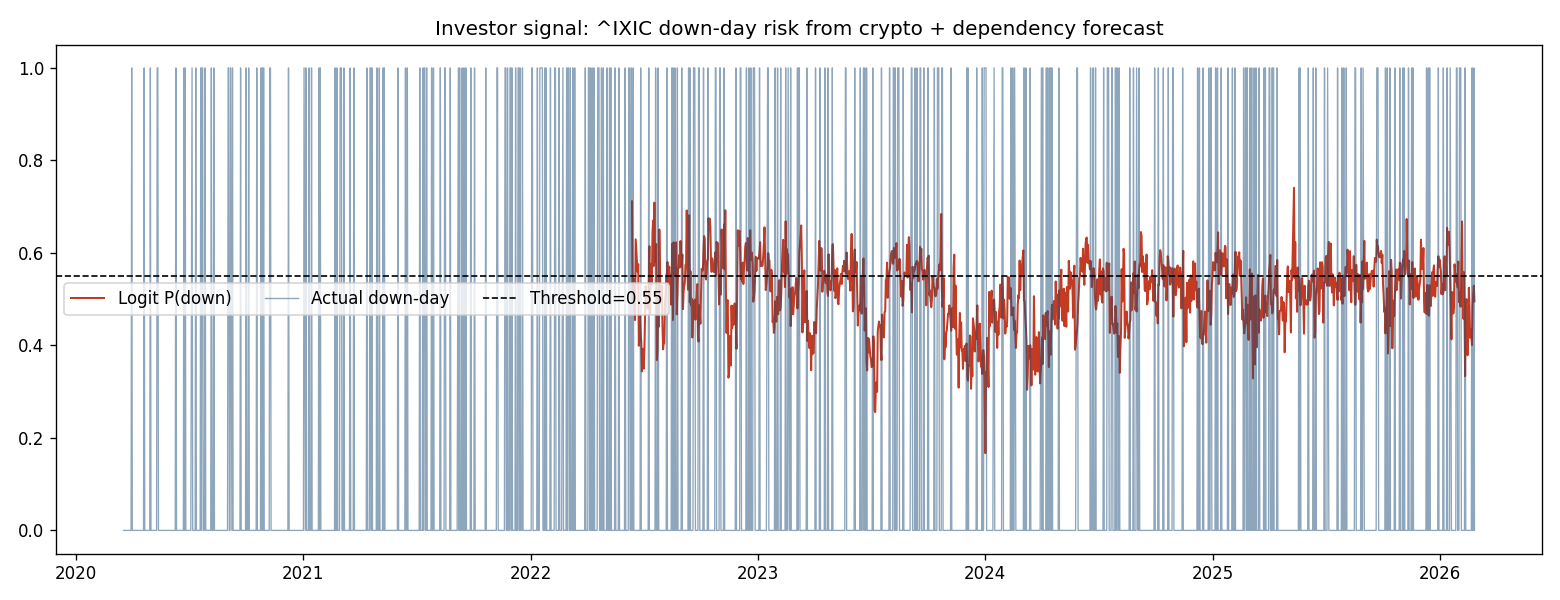
\includegraphics[width=0.9\textwidth]{../outputs/figures/signal_corr_BTC-USD_^IXIC_w30.png}
    \caption{Signal-layer output for the Bitcoin--NASDAQ relation at the 30-day window.}
\end{figure}

\begin{figure}[H]
    \centering
    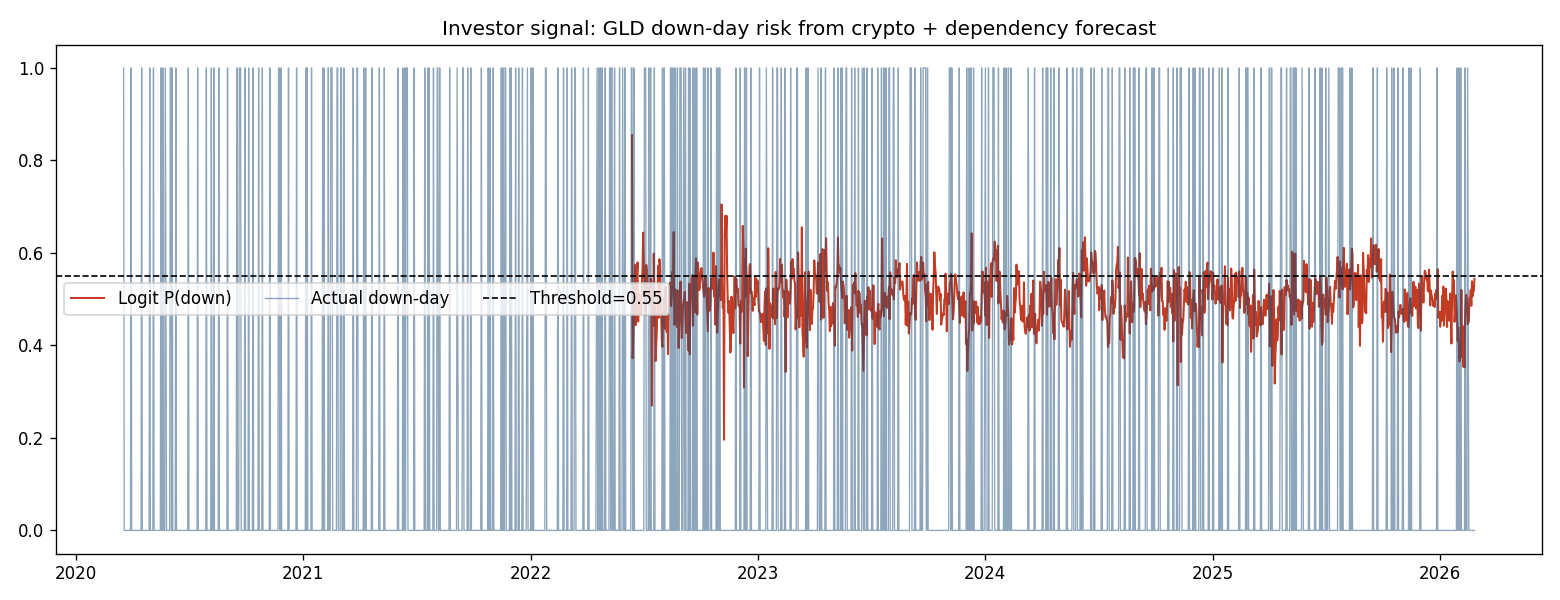
\includegraphics[width=0.9\textwidth]{../outputs/figures/signal_corr_BTC-USD_GLD_w30.png}
    \caption{Signal-layer output for the Bitcoin--gold relation at the 30-day window.}
\end{figure}

\begin{figure}[H]
    \centering
    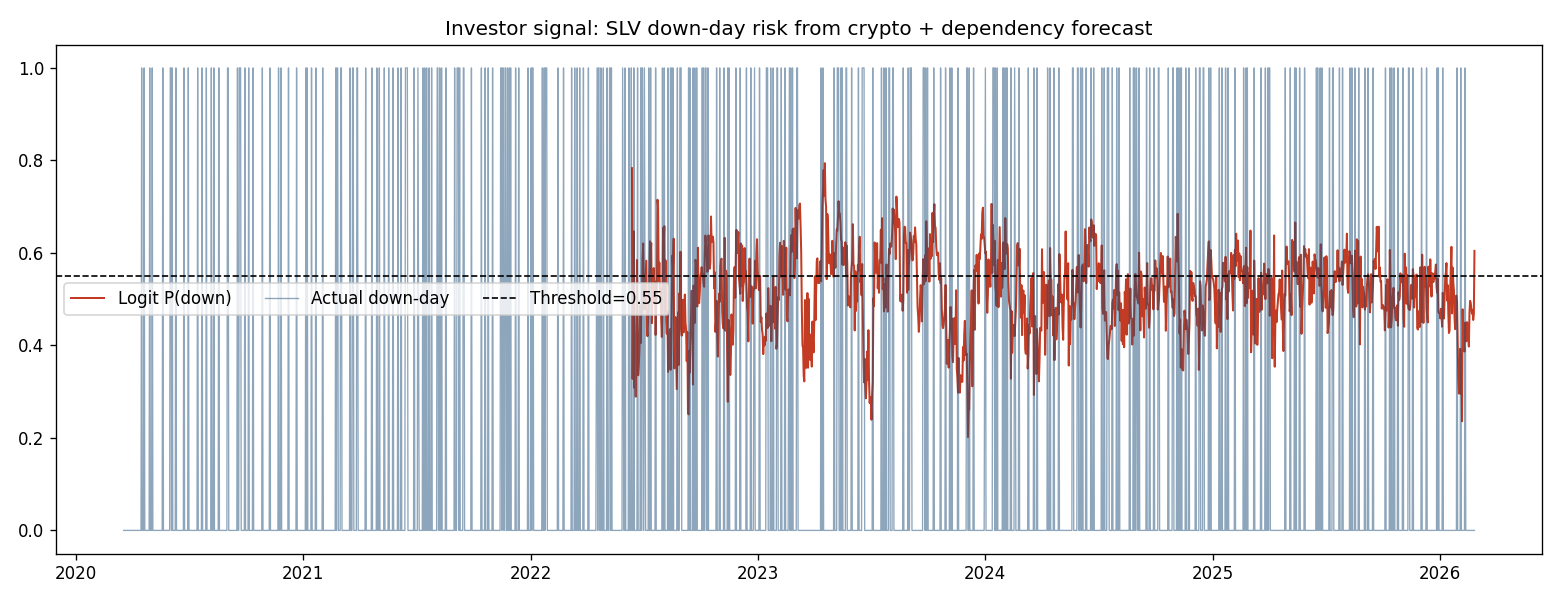
\includegraphics[width=0.9\textwidth]{../outputs/figures/signal_corr_BTC-USD_SLV_w30.png}
    \caption{Signal-layer output for the Bitcoin--silver relation at the 30-day window.}
\end{figure}

\begin{figure}[H]
    \centering
    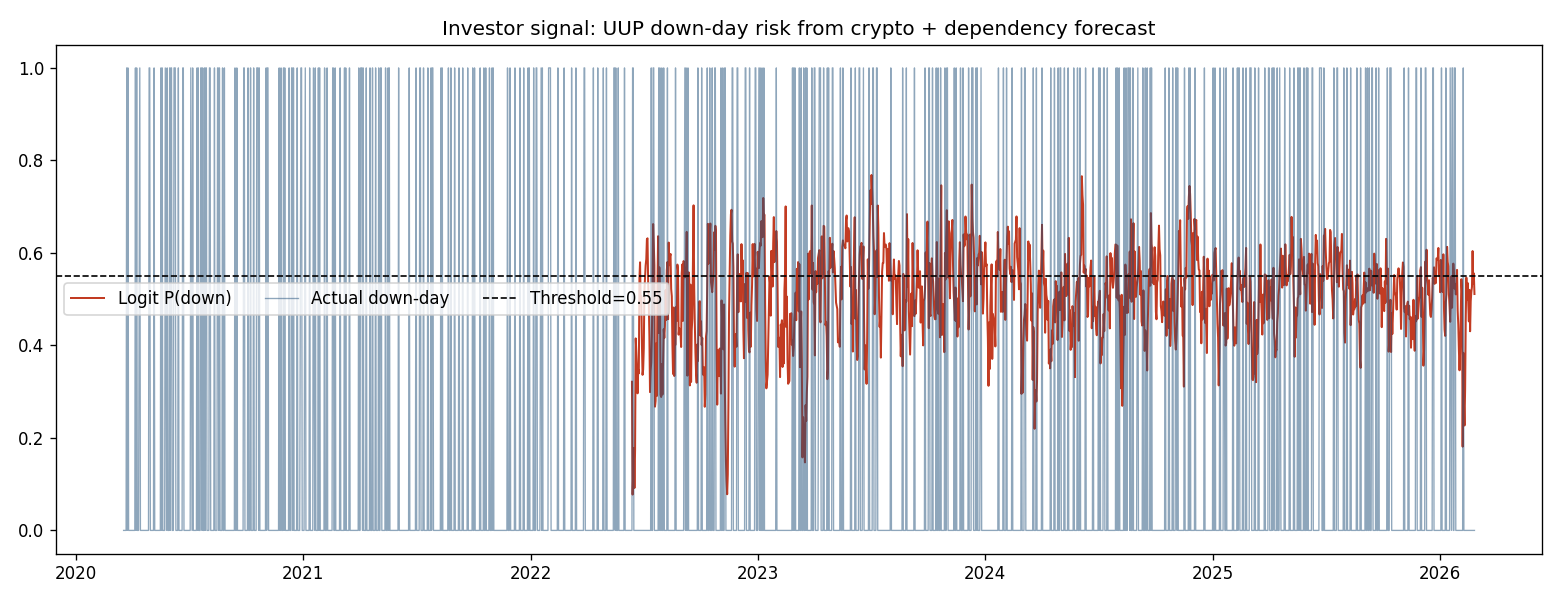
\includegraphics[width=0.9\textwidth]{../outputs/figures/signal_corr_BTC-USD_UUP_w30.png}
    \caption{Signal-layer output for the Bitcoin--UUP relation at the 30-day window.}
\end{figure}

\subsection{Cross-market warning interpretation}

The supplementary signal figures show that the practical layer behaves differently across markets. Equity-related targets display somewhat clearer warning episodes, while the metal and dollar-linked targets are noisier and weaker. This asymmetry is economically sensible and supports the interpretation that the investor layer should be used selectively rather than uniformly.

\subsection{Summary table}

\begin{table}[H]
    \centering
    \caption{Average signal-layer performance by classifier family.}
    \begin{tabular}{lrrr}
        \toprule
        Signal model & Balanced Accuracy & F1\_down & AUC \\
        \midrule
        Logit & 0.506 & 0.209 & 0.508 \\
        GBM\_Cls & 0.501 & 0.033 & 0.520 \\
        RF\_Cls & 0.500 & 0.030 & 0.519 \\
        \bottomrule
    \end{tabular}
\end{table}

These summary values confirm that the signal layer is meaningful but modest. Its strongest role is as a supplementary warning mechanism rather than as a standalone allocator.

\clearpage
\begin{figure}[p]
    \centering
    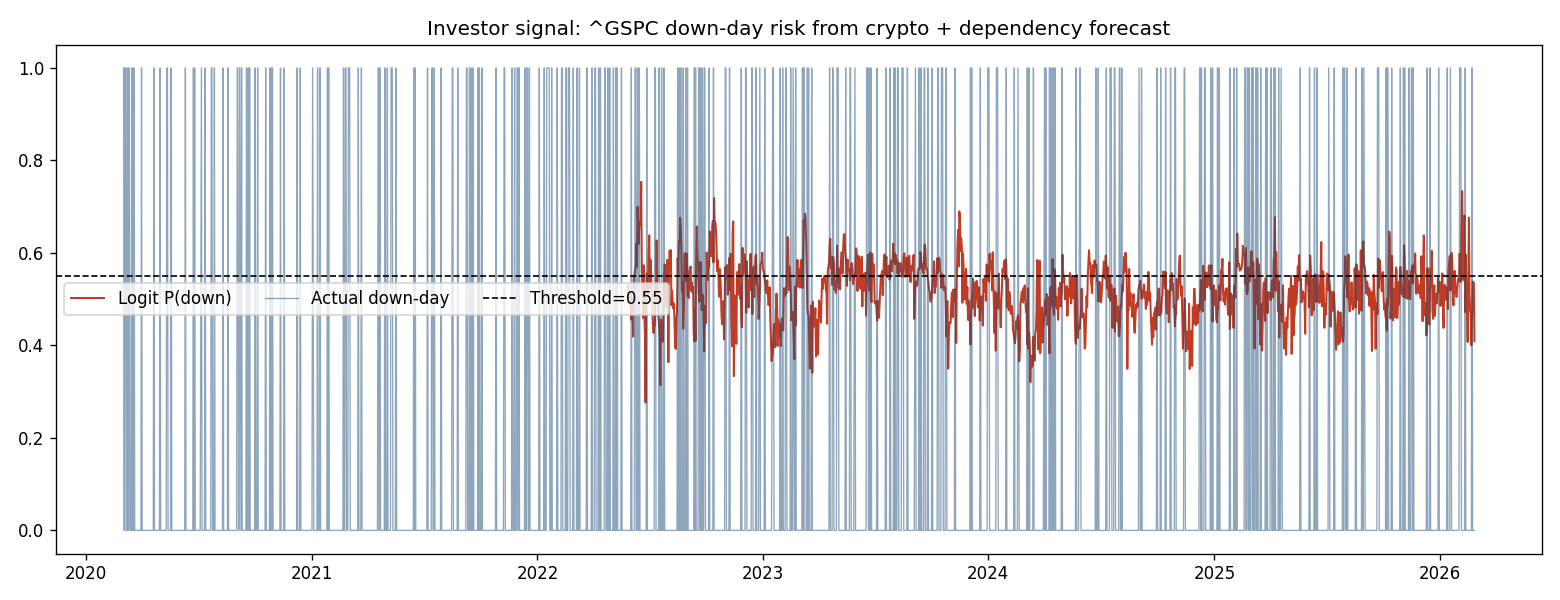
\includegraphics[width=0.95\textwidth]{../outputs/figures/signal_corr_BTC-USD_^GSPC_w14.png}
    \caption{Supplementary S\&P 500 warning signal at the 14-day window.}
\end{figure}

\clearpage
\begin{figure}[p]
    \centering
    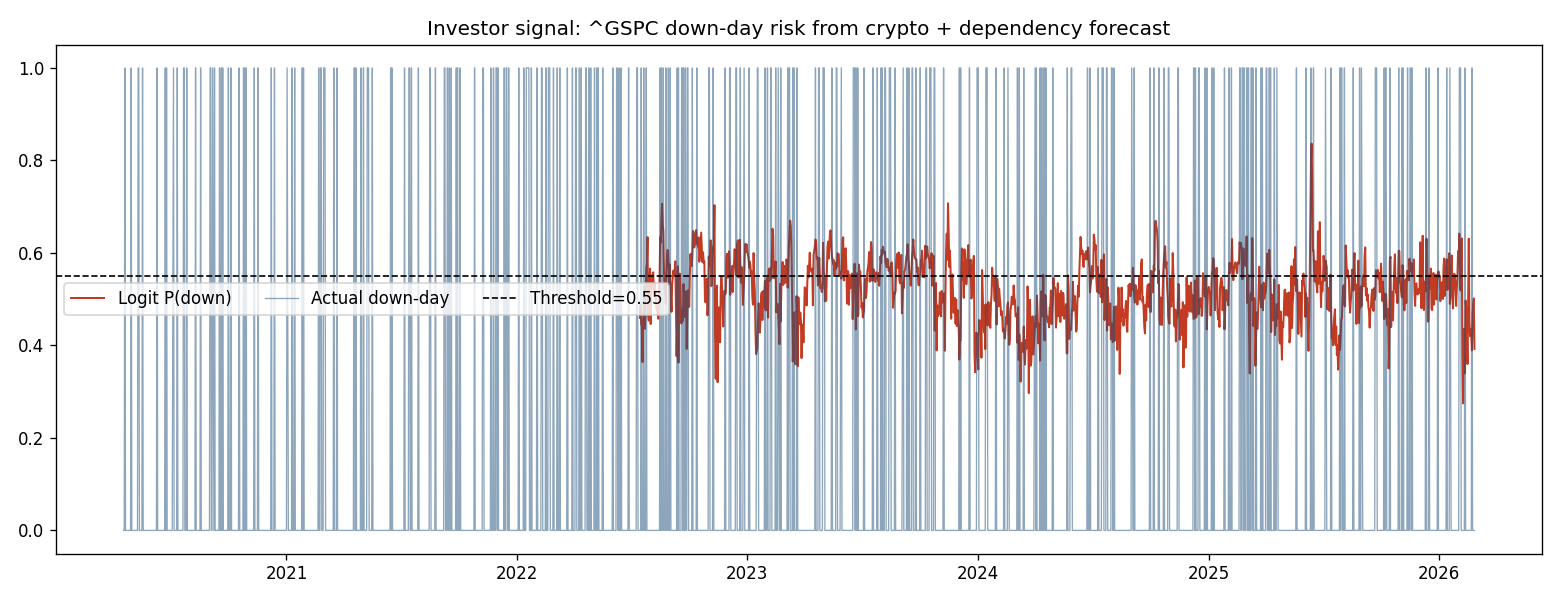
\includegraphics[width=0.95\textwidth]{../outputs/figures/signal_corr_BTC-USD_^GSPC_w60.png}
    \caption{Supplementary S\&P 500 warning signal at the 60-day window.}
\end{figure}

\clearpage
\begin{figure}[p]
    \centering
    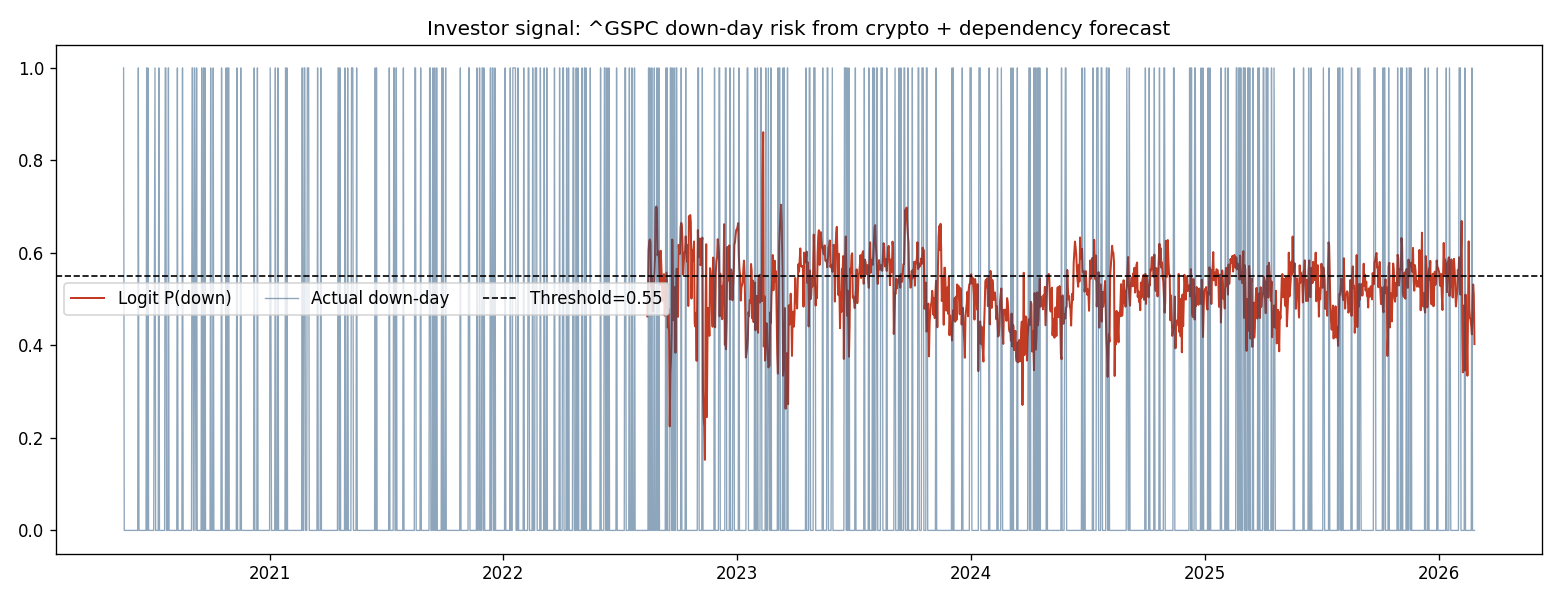
\includegraphics[width=0.95\textwidth]{../outputs/figures/signal_corr_BTC-USD_^GSPC_w90.png}
    \caption{Supplementary S\&P 500 warning signal at the 90-day window.}
\end{figure}

\clearpage
\begin{figure}[p]
    \centering
    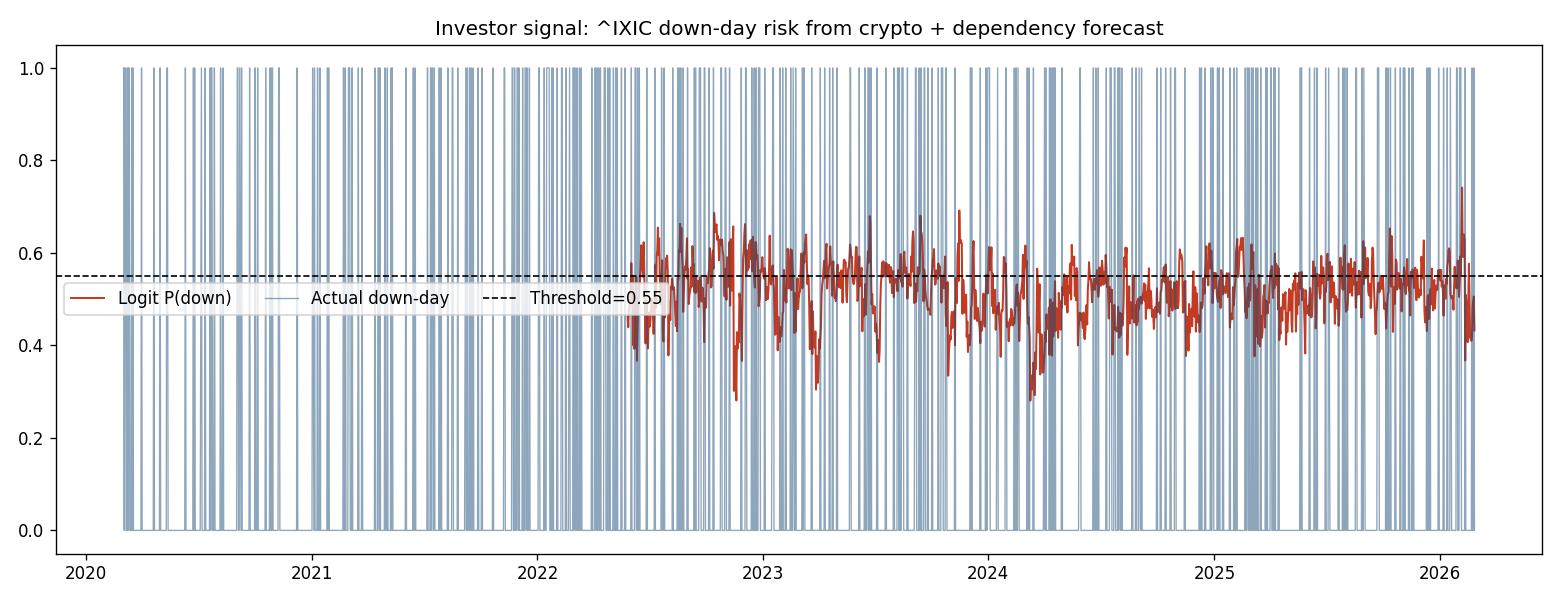
\includegraphics[width=0.95\textwidth]{../outputs/figures/signal_corr_BTC-USD_^IXIC_w14.png}
    \caption{Supplementary NASDAQ warning signal at the 14-day window.}
\end{figure}

\clearpage
\begin{figure}[p]
    \centering
    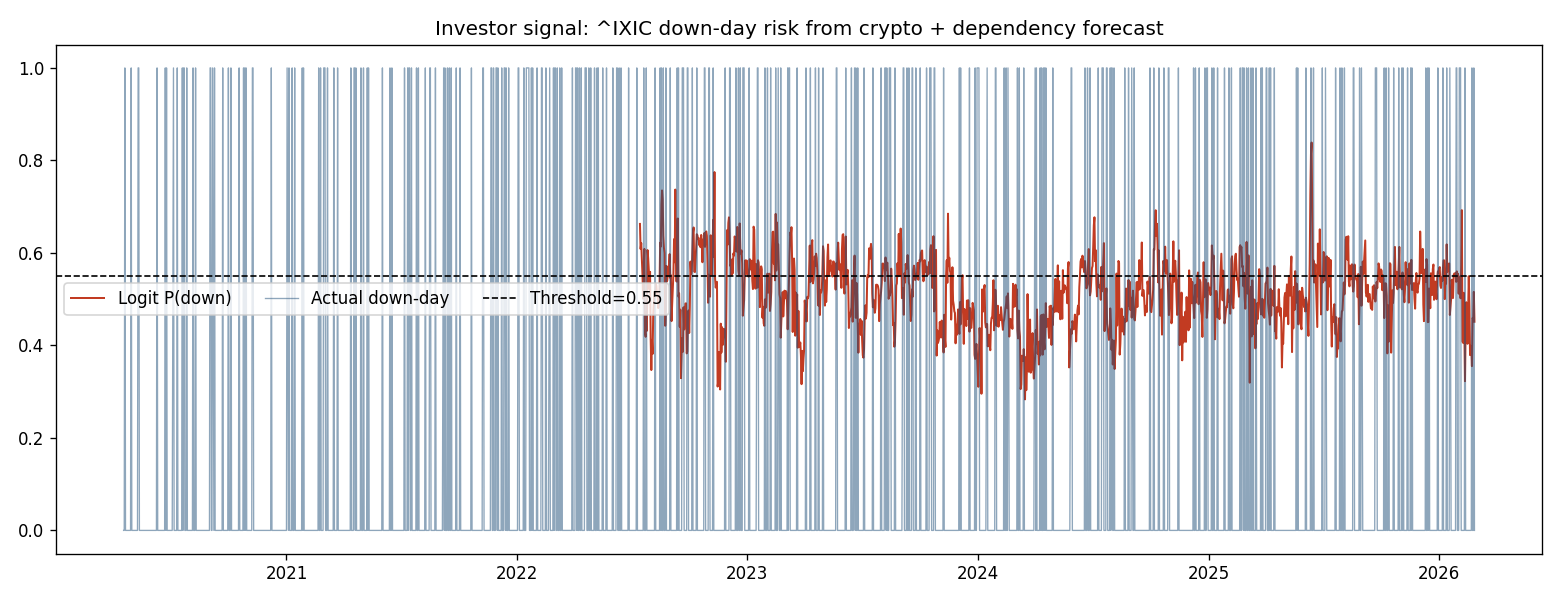
\includegraphics[width=0.95\textwidth]{../outputs/figures/signal_corr_BTC-USD_^IXIC_w60.png}
    \caption{Supplementary NASDAQ warning signal at the 60-day window.}
\end{figure}
